% Chapter 1
\chapter{Introducción general} % Main chapter title

\label{Chapter1} % For referencing the chapter elsewhere, use \ref{Chapter1} 
\label{IntroGeneral}

%----------------------------------------------------------------------------------------

% Define some commands to keep the formatting separated from the content 
\newcommand{\keyword}[1]{\textbf{#1}}
\newcommand{\tabhead}[1]{\textbf{#1}}
\newcommand{\code}[1]{\texttt{#1}}
\newcommand{\file}[1]{\texttt{\bfseries#1}}
\newcommand{\option}[1]{\texttt{\itshape#1}}
\newcommand{\grados}{$^{\circ}$}

%----------------------------------------------------------------------------------------

%\section{Introducción}

%----------------------------------------------------------------------------------------
\section{Estaciones transformadoras}

Se denomina estación transformadora al conjunto de equipos electromecánicos responsables de convertir la energía eléctrica variando uno o más de sus principales parámetros, que son tensión y corriente. Esta conversión se logra a través del componente más importante del conjunto, el transformador. La finalidad de convertir la energía eléctrica, que puede ser elevando o reduciendo el nivel de tensión, es poder transmitir y distribuir esa energía hacia los receptores que pueden ser consumidores finales tales como residencias familiares o polos industriales.\\

Por convención se denomina Estación Transformadora (E.T.) cuando en el proceso se ven involucrados valores considerados de alta tensión (mayor a 66 kV) y Subestación Transformadora (S.E.T.) en el caso de tensiones menores a 66 kV \citep{AEA:1}.\\
Para la distribución hacia los consumidores finales, se utilizan las denominadas Subestaciones Transformadoras Aéreas (S.E.T.A.) que convierten la tensión disminuyendo su valor de media a baja tensión.\\

Para poder obtener energía eléctrica a la salida en óptimas condiciones de calidad y disponibilidad, resulta fundamental administrar y controlar los valores intrínsecos que componen la transmisión y recepción de la misma. Esto se logra a través de instrumentos de medición de tensión y corriente, tanto a la entrada (alta tensión) como a la salida (media tensión) de la conversión. Por otro lado, con el fin de mantener y preservar los equipos electromecánicos se consideran de gran importancia otros valores físicos como temperatura y humedad.\\
\section{Medidores de energía}
Llegado el momento de entregar la energía al usuario final, es indispensable cuantificarla para luego comercializarla. Las distribuidoras del servicio utilizan medidores de energía electromecánicos o electrónicos, que registran en todo momento la energía acumulada que fluye por el mismo.\\
La medición de corriente puede ser directa, vinculando los conductores de alimentación de la carga directamente al medidor o indirecta. Una medición indirecta consiste en reducir los valores de corriente de carga a través de transformadores de corriente (TI) y vincular sus secundarios al medidor \ref{fig:medicioncorrienteconti}. Este último método se emplea en casos donde la corriente calculada supera el valor permitido por el medidor de energía, por lo que es necesario multiplicar el valor de la lectura por un coeficiente correspondiente a la relación de transformación del TI.\\

% TODO: \usepackage{graphicx} required
\begin{figure}
	\centering
	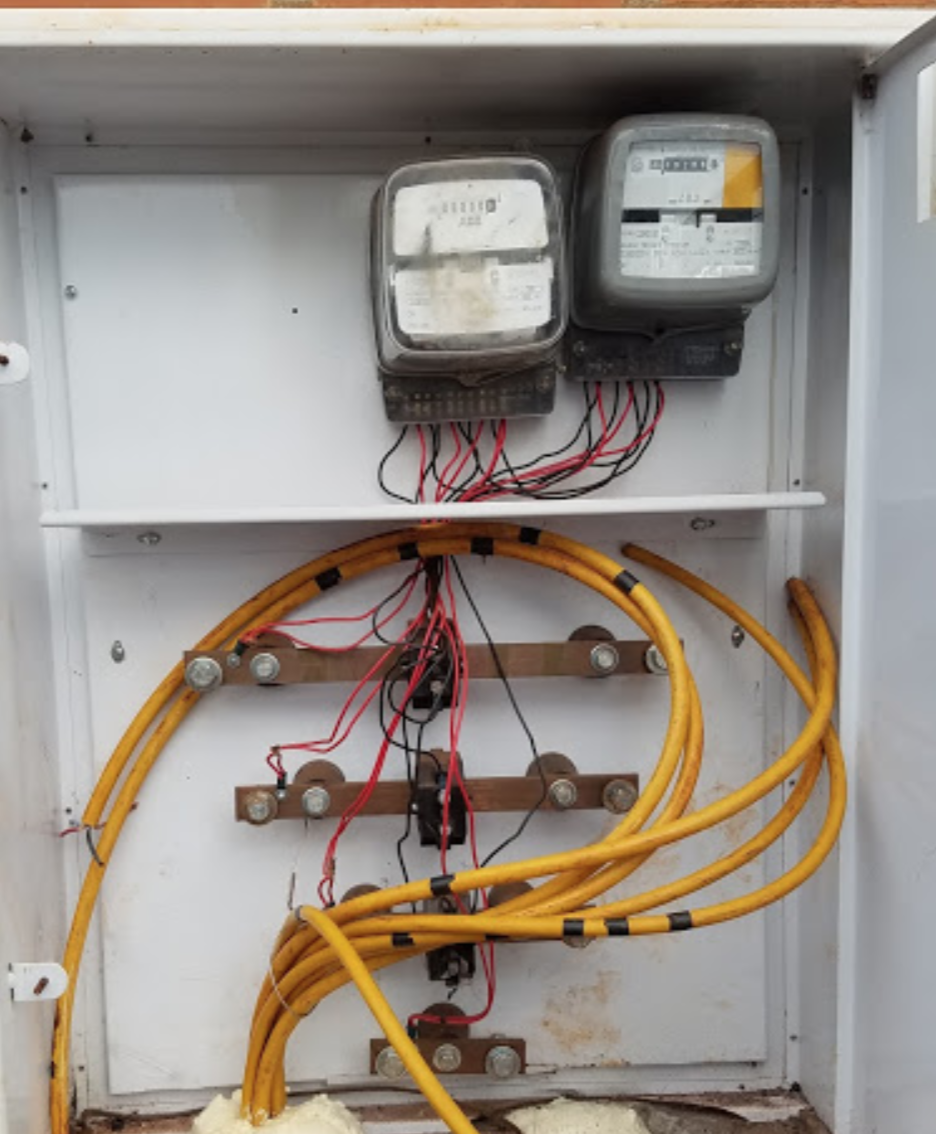
\includegraphics[width=0.5\linewidth]{Figures/Medicion_corriente_con_TI}
	\caption[]{Medición indirecta de corriente empleando transformadores de corriente (TI).\protect\footnotemark}
	\label{fig:medicioncorrienteconti}
\end{figure}
\footnotetext{Imagen tomada por el autor}

% TODO: \usepackage{graphicx} required
\begin{figure}
	\centering
	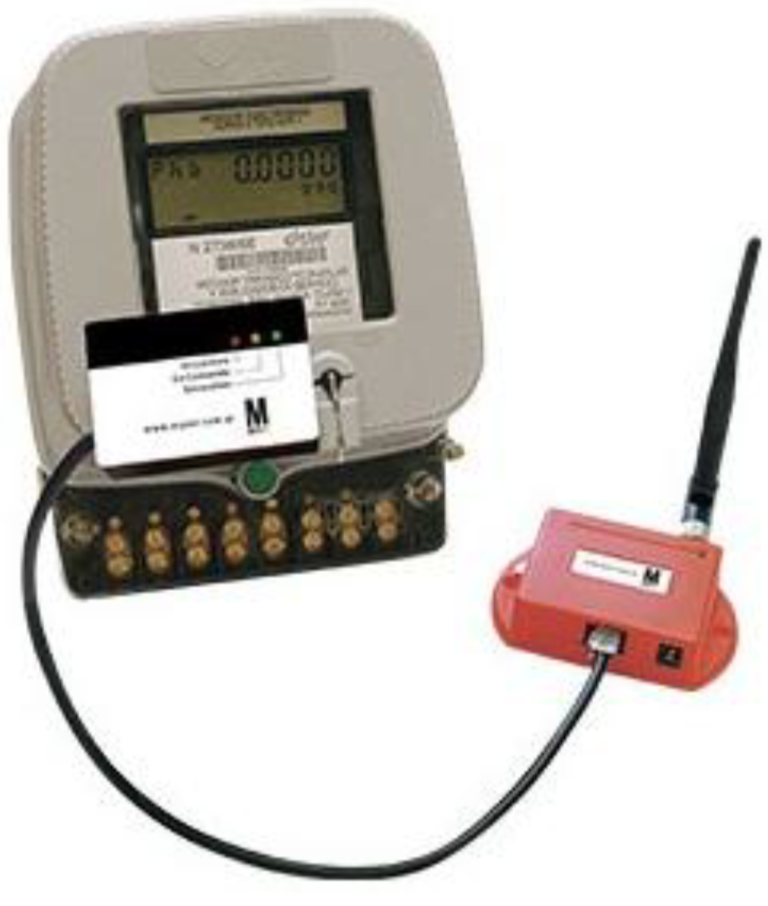
\includegraphics[width=0.5\linewidth]{Figures/medidor_digital_con_complemento_gsm}
	\caption{Medidor de energía digital con complemento para telemedición mediante GSM. Imagen tomada de \citep{MYEEL}}
	\label{fig:medidordigitalconcomplementogsm}
\end{figure}
En la actualidad algunas prestadoras del servicio eléctrico han adoptado estrategias de medición inteligente similares a la presentada en la figura \ref{fig:medidordigitalconcomplementogsm}. En este esquema los equipos de medición se reportan a centros de operación a través de una red de comunicaciones móvil, como por ejemplo GSM.\\
El concepto de telemedición aporta además de lo comercial, valiosa información técnica, ya que los centros de operaciones conocen en todo momento el estado del medidor con la posibilidad de detectar fallas o la interrupción del servicio eléctrico.\\  

\section{Estado del arte y problemática identificada}
En Sudamérica, gran parte de las empresas distibuidoras de energía eléctrica y sus tercerizadas, basan parte de sus operaciones en el contacto directo con los usuarios finales mediante reclamos para informarse acerca de interrupciones en el servicio de distribución de energía eléctrica. Una vez recibido un reclamo, la prestadora de servicios envía al grupo de operaciones especializado a recorrer el área circundante al cliente y tratar de determinar el motivo de la interrupción del servicio.\\

% TODO: \usepackage{graphicx} required
\begin{figure}[h!]
	\centering
	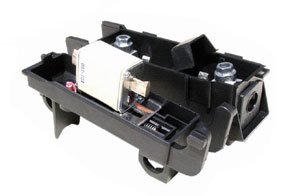
\includegraphics[width=0.7\linewidth]{Figures/NH_aereo_bt}
	\caption{Fusible seccionador aéreo tipo NH usualmente utilizado en lineas de distribución de baja tensión}
	\label{fig:nh_aereo_bt}
\end{figure}
Un hecho común en el nordeste Argentino y particularmente en la provincia de Misiones es la destrucción de fusibles aéreos como el presentado en la figura \ref{fig:nh_aereo_bt}. Estos fusibles conectados inmediatamente a la salida de baja tensión y en serie con las líneas de distribución, cumplen la función de protección por sobrecorriente debido a picos de consumo o cortocircuitos causados por desastres naturales como el de la figura \ref{fig:arbolcaidolineabt}. Los fusibles involucrados actúan de manera correcta autodestruyendose e interrumpiendo el paso de corriente.\\
Este esquema presentado, resulta aún precario y no efectivo en cuanto a la rapidez para determinar la localización geográfica donde se ha generado una falla, lo que resulta en una inferior calidad de servicio prestado al cliente.\\
\begin{figure}[h!]
	\centering
	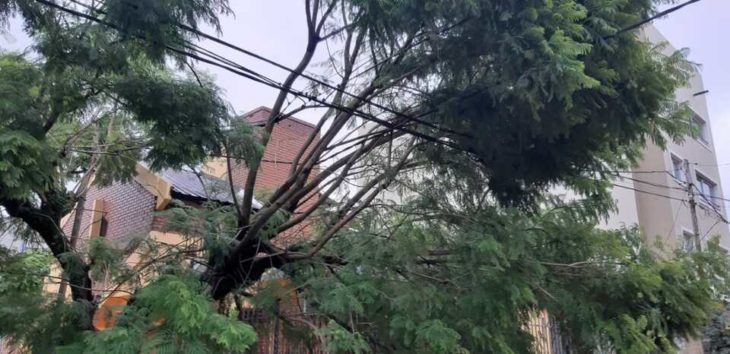
\includegraphics[width=0.7\linewidth]{Figures/arbol_caido_linea_bt}
	\caption{Un árbol caído sobre las líneas de distribución aéreas de baja tensión luego de una breve tormenta en la ciudad de Posadas, Misiones. Imagen tomada de \citep{Noticia_MNES}}
	\label{fig:arbolcaidolineabt}
\end{figure}

Cabe mencionar que la mayoría de las redes de distribución de baja tensión en 380/220V no poseen la capacidad de brindar algún otro servicio agregado. Como una manera de previsión a la necesidad de montar servicios adicionales a las redes de transmisión de media y alta tensión (33 kV y 132 kV), a las redes propias de transmisión de energía, se adiciona una infraestructura de fibra óptica, por medio de un cable de guarda aéreo compuesto de acuerdo a estándares de IEEE (OPGW - Optical Fiber Composite Overhead Ground Wire-). Ésta instalación combina las funciones de conexión a tierra y de comunicaciones, estableciendo una estructura tubular de varios pares de fibras ópticas en el mismo, rodeadas por capas de hilos de aluminio y acero. La parte conductora del cable sirve para unir las puestas a tierra de las estructuras adyacentes, protegiendo a estas de las descargas atmosféricas.\\
Las fibras ópticas dentro del cable se utilizan para la transmisión de datos a alta velocidad, ya sea para uso propio del sistema eléctrico de protección y control de la línea de transmisión, para la comunicación de voz y datos, o pueden ser alquilados o vendidos a terceros para servir como una interconexión de fibra de alta velocidad entre diferentes ciudades. En ciertas ocasiones, frente a condiciones climáticas extremas éstas instalaciones muestran cierta vulnerabilidad, conllevando a un elevado costo de mantenimiento \citep{ARTICLE:1}.\\
Lu, Liang, Li y Guo \citep{ARTICLE:1} y Sosa y Sosa \citep{ARTICLE:2}, comparten la aplicación de un modelo de arquitectura de 3 capas para los sistemas smart grid: física, red y aplicación. Definiendo donde residirá la aplicación y su objetivo final, surgen diferentes estrategias de control a ser implementadas. De la misma manera, la selección de sensores de diferente tipo (meteorológicos, estructurales, operacionales, etc.) residen en entornos controlados, los cuales se establecen mediante el despliegue e implementación de redes de diferente tecnología y modos de comunicación.\\
Las tecnologías emergentes propias de IoT tales como las redes de comunicación de baja potencia y largo alcance LPWAN \citep{rfc8376}, y las redes tipo malla se consideran como tecnologías disponibles y viables para proveer una infraestructura de comunicaciones a las redes de distribución metropolitanas  \citep{ARTICLE:4}. Otros autores presentan sistemas de medición de temperatura autónomos utilizando transductores termoeléctricos y electromagnéticos para la conversión de energía térmica o electromagnética en energía eléctrica utilizada para alimentar la electrónica involucrada y acumuladores \citep{ARTICLE:5}, \citep{Hua}.

%----------------------------------------------------------------------------------------

\section{Objetivos y alcance}
\subsection{Objetivo general}
Desarrollar un sistema capaz de determinar valores eficaces de corriente alterna en sistemas metropolitanos de distribución de energía eléctrica en baja tensión y reportar estados a un centro de operaciones a través de una red LoRaWAN de acceso público.\\
\subsection{Objetivos específicos}
\begin{itemize}
	\item Evaluar el uso de un supercapacitor como reemplazo de una batería convencional.\\
	\item Desarrollar una electrónica de ultra bajo consumo para maximizar la autonomía de operación del supercapacitor.
\end{itemize}
\subsection{Alcances}
En el presente proyecto se desarrollan los siguientes temas:
\begin{itemize}
	\item Circuito de conversión de energía  basado en rectificadores de alta eficiencia.
	\item Acumulador de energía basado en supercapacitores
	\item Patrón de firmware implementado en el microcontrolador para optimizar el uso de energía del acumulador.
	\item Medición de valor RMS de corriente mediante transformador de corriente.
	\item Tecnología LoRaWAN.
	\item Recuperación, almacenamiento y presentación de datos generados por los nodos finales.
\end{itemize}
Si bien el proyecto es parte de un plan de creación de una PyME del autor, no es parte del alcance ni se cubren en este documento las etapa de lanzamiento de producto ni creación de la empresa.
